\clearpage
\section{Experimentos e Resultados} \label{sec:exp_result}

Este capítulo apresenta os experimentos realizados para a avaliação da proposta \system detalhada na Seção~\ref{sec:methods} e discute os resultados obtidos.
Foram avaliados diversos cenários, sempre considerando o conjunto de dados \dataset e sua segmentação realizada por especialistas.
Em um primeiro momento buscou-se definir quais são os parâmetros mais adequados para a abordagem \system, assim como quantificar o impacto da mudança nesses parâmetros na segmentação final.
As Seções~\ref{sec:exp_amostragem},~\ref{sec:exp_classificacao} e~\ref{sec:exp_dbcscan} apresentam os experimentos realizados com a finalidade de determinar quais são os melhores parâmetros para a solução proposta, enquanto as Seções~\ref{sec:exp_amostragem} e~\ref{sec:exp_dbcscan_2} quantificam o impacto de cada uma das etapas do método com relação ou ao tempo de processamento ou ao resultado esperado.
Em um segundo momento, foi realizada uma avaliação comparativa entre a segmentação automática realizada pela solução \system contra um pequeno conjunto de imagens segmentado manualmente por um especialista do domínio.
A segmentação automática foi realizada de acordo com o melhor conjunto de parâmetros determinado pelos experimentos anteriores e conseguiu alcançar uma taxa de sucesso comparadas a do especialista, como é relatado na Seção~\ref{sec:exp_vs_especialista}.

A primeira etapa do processo de avaliação consistiu na definição do conjunto de dados rotulado para o treinamento do classificador da primeira fase do \system.
Na sequência, diversos classificadores foram avaliados para o processamento do conjunto de dados rotulados, sendo empregadas diversas métricas de qualidade para definir a melhor abordagem de classificação.
Os próximos experimentos foram realizados para determinar os parâmetros mais adequados para a execução do algoritmo DBSCAN.
Em particular, foram avaliadas cinco funções de distância que possuem diferentes perspectivas geométricas e o resultado foi quantificado em função do limite de similaridade máximo tolerado pelo DBSCAN.
O último exame sobre a qualidade da proposta foi usar o método \system com o melhor classificador, com o melhor limite de similaridade e melhor função de distância (todos obtidos experimentalmente) para segmentar imagens reais do conjunto \dataset, sendo que o resultado obtido foi justaposto à segmentações manuais realizada por um especialista.

Todos os experimentos foram realizados em uma máquina local com a seguinte seguinte configuração: Sistema Operacional Linux Ubuntu 18.04.1 LTS\footnote{\url{releases.ubuntu.com/18.04/}} com um processador $i3 - 2310M  ~ 2.1$ Ghz de $04$ núcleos, equipado com 06Gb de memória RAM.
Os conjuntos de dados avaliados e/ou gerados para a definição da parametrização do sistema se encontram publicamente disponíveis no mesmo repositório do código-fonte da solução\footnote{\url{github.com/sswellington/2PLA/tree/master/dataset}}.

\subsection{Definição dos parâmetros para a primeira fase do \system} \label{sec:exp_amostragem}	

O primeiro ponto a ser definido para a escolha dos parâmetros adequados da proposta \system é o uso de um conjunto de dados rotulado para o treinamento da fase de classificação.
Nesse sentido, combinou-se, manualmente, as segmentações das úlceras definidas pelos especialistas no \textit{ground-truth} do conjunto de dados \dataset e os limites de pele saudável para determinar os pixels que fazem parte do plano de fundo das imagens.
Para gerar o conjunto de dados, foram separadas dez imagens do conjunto \dataset diversificadas entre si.
Essas imagens \textit{não foram usadas em nenhum dos próximos experimentos}, com o objetivo de se testar instâncias (imagens) de forma isolada e independente do processo de treinamento.


Após essa separação manual dos pixels de plano de fundo com a definição de pontos de fronteira, os pixels das $10$ imagens tomadas como exemplos foram divididos em duas classes $L= \{$Pele,Fundo$\}$.
A Figura~\ref{fig:sample} apresenta exemplos dessas duas classes para mesmas imagens.
Esse processo resultou na geração de mais de 100 milhões de pixels que foram armazenados em arquivos separados por vírgula (\texttt{.CSV}) e rotulados de forma desbalanceada, pois existiam nas imagens originais mais pixels da classe Fundo do que da classe Pele.
Em particular, os pixels armazenados apresentaram a proporção de $4/7$ de pixels de ``Fundo'' e $3/7$ de pixels de ``Pele''.
Essa quantidade de instâncias inviabiliza o procedimento de treino de classificadores em uma única máquina centralizada, devido ao custo computacional e ao tempo hábil para a execução de alguns viéses de algoritmos de aprendizado. 

\begin{figure}[!htb]
\centering
\includegraphics[scale=1]{_fig/sample.pdf}
\caption[Exemplos de pixels rotulados entre $L= \{$Pele,Fundo$\}$]{Exemplos de pixels rotulados entre $L= \{$Pele,Fundo$\}$.}
\label{fig:sample}
\end{figure}

Nesse sentido, foi necessário o uso de técnicas de amostragem sobre o conjunto de dados coletado.
Como o conjunto apresenta rótulos, optou-se por usar uma amostragem aleatória \textit{estratificada} sem reposição, onde pixels da mesma classe tiveram a mesma chance de ser escolhidos e a amostra resultante respeita a proporção de $4/7$ e $3/7$ de pixels por classe encontradas no conjunto rotulado original.
Além disso, optou-se por extrair amostras de diversas granularidades ao invés de um único conjunto, com o objetivo de compreender como o algoritmo de aprendizado aderia ao conjunto amostral.
Nesse sentido, foram extraídas amostras de crescentes cardinalidades com os valores de $1 \cdot 10^1, 1 \cdot 10^2, 1 \cdot 10^3, 1 \cdot 10^4$ e $1 \cdot 10^5$ pixels.
A amostra de tamanho $1 \cdot 10^1$ está contida na amostra de tamanho $1 \cdot 10^2$ e assim, sucessivamente.

Antes da aplicação do algoritmo de aprendizagem, os pixels das amostras foram visualizados por meio de um gráfico de pontos em três dimensões, onde cada dimensão é um eixo do modelo de cores RGB que varia no intervalo $[0, 255]$.
A Figura~\ref{fig:plot} apresenta os gráficos para os três maiores tamanhos de amostras: $1 \cdot 10^3, 1 \cdot 10^4$ e $1 \cdot 10^5$, onde os pontos são divididos em dois grupos de cores diferentes.

Para cada uma das amostras, pode-se verificar que os pontos se encontram ligeiramente separados.
Para a amostra de menor cardinalidade eles se separam por um plano e para as duas de maior cardinalidade, por múltiplos planos concatenados.
Em alguns trechos, as classes se confundem, ou devido à \textit{outliers} (valores extremos) ou à característica não espacialmente uniforme do modelo de cores RGB.
Além disso, é possível verificar uma ligeira separação dentro da classe ``Fundo'' presente nos três tamanhos de amostras.
Essa separação é devido a tonalidade presente nos planos de fundo que são ou ``azuis'' ou ``brancos''.

\begin{figure}[!htb]
\centering
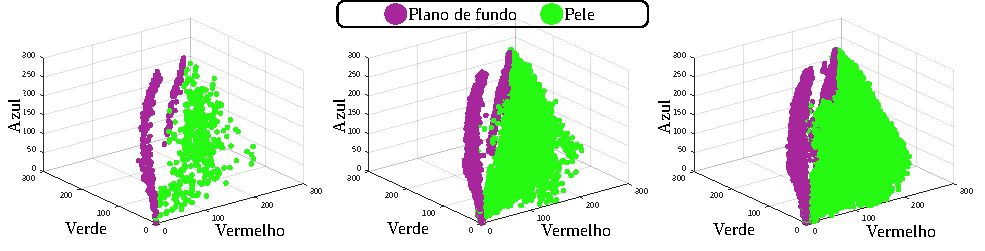
\includegraphics[scale=.92]{_fig/plots.pdf}
\caption[Amostra de pixels rotulados no modelo RGB]{Amostra de pixels rotulados no modelo RGB.
Tamanho (cardinalidade) das amostras visualizadas:
(a)~$1 \cdot 10^3$,
(b)~$1 \cdot 10^4$, e
(c)~$1 \cdot 10^5$.}
\label{fig:plot}
\end{figure}

Dado esse contexto do conjunto de dados, alguns paradigmas de aprendizado parecem mais adequados como candidatos com melhor aderência ao conjunto de dados.
Em particular, aqueles baseados em hiper-planos e hiper-retângulos parecem candidatos capazes de separar as duas classes.
Assim, esses algoritmos foram avaliados sobre todas as cardinalidades de amostras geradas no experimento em sequência.

\subsection{Avaliação de classificadores para a primeira fase do \system} \label{sec:exp_classificacao}

Dadas as características do problema, avaliou-se um conjunto de classificadores como candidatos à primeira fase da proposta \system.
Em particular, experimentou-se sobre os métodos de classificação estatísticos Na\"ive-Bayes e Bayes-Net, baseado em instâncias \textit{$k$-Nearest Neighbor} (kNN), conexionista \textit{Multi-Layer Perceptron} (MLP) e simbólicos \textit{DecisionTree}, \textit{RandomTree} e \textit{RandomForest}.
Todos os classificadores foram usados de acordo com a sua implementação na ferramenta \textit{Weka}, com a seguintes configurações:

\begin{itemize}
    \item \underline{Na\"ive-Bayes}: Não requer parâmetros,
    \item \underline{Bayes-Net}: Grafo de correlação apenas entre pares de dimensões, com busca heurística \textit{Hill-Climbing},
    \item \underline{kNN}: Um vizinho mais próximo, com função de distância $L_2$,
    \item \underline{MLP}: Rede totalmente conectada, com três neurônios na camada de entrada com função de ativação de minmax, uma camada escondida, com dois neurônios com função de ativação logística, dois neurônios na camada de saída com função de ativação minmax, toda a rede com topologia \textit{backpropagation} treinada ou pelo algoritmo de Levenberg-Marquardt (LM) ou pelo algoritmo Resilient Propagation (RPROP),
    \item \underline{DecisionTree}: Árvore apenas binária, com critério de Gini e com poda,
    \item \underline{RandomTree}: Sem limite de profundidade ou número de elementos por folha,
    \item \underline{RandomForest}: Cem iterações e cinco árvores,
\end{itemize}

Para avaliar esses classificadores foi realizado um procedimento de validação cruzada de $10$-folds.
Portanto, o conjunto de treinamento foi dividido, de forma estratificada, em $10$ porções e, para cada uma das $10$ iterações, nove porções foram usadas como conjunto de treinamento e uma como conjunto de teste.
Assim, os valores de qualidade são tomados como \textit{médias} sobre as $10$ matrizes de confusão obtidas ao final do procedimento de validação cruzada.
Ainda nesse sentido, para demonstrar o poder discriminativo dos métodos de classificação, incluímos o método de limiarização de Otsu como mais um \textit{possível candidato} à primeira fase da solução \system.
O método de limiarização é um classificador que usa apenas um ponto de corte.

\begin{table}[!b]
\centering
\caption[Coeficiente de Cohen--Kappa como a qualidade do classificador da primeira fase da solução \system]{Coeficiente de Cohen--Kappa como a qualidade do classificador da primeira fase da solução \system. 
Os valores numéricos $[-1,1]$ podem ser interpretados semanticamente de acordo com a Figura~\ref{fig:kappa} da Seção~\ref{sec:background}.}
\label{tab:classifiersCKC}
\begin{tabular}{l|c|c|c|c|c||c|c} \hline \hline
 & 
\multicolumn{7}{c}{ {\cellcolor[HTML]{68CBD0}\textbf{Tamanho da Amostra}} }    \\ \hline
\cellcolor[HTML]{68CBD0} \textbf{Classificador} & 
\cellcolor[HTML]{68CBD0} \textbf{$1 \cdot 10^1$}  & 
\cellcolor[HTML]{68CBD0} \textbf{$1 \cdot 10^2$}  & 
\cellcolor[HTML]{68CBD0} \textbf{$1 \cdot 10^3$}  & 
\cellcolor[HTML]{68CBD0} \textbf{$1 \cdot 10^4$}  & 
\cellcolor[HTML]{68CBD0} \textbf{$1 \cdot 10^5$}  &
\cellcolor[HTML]{68CBD0} \textbf{$\bar{\mu}$} &
\cellcolor[HTML]{68CBD0} \textbf{$\mu$}\\ \hline \hline
Na\"ive-Bayes         & 0,156 & 0,710 & 0,793 & 0,797 & 0,805  & 0,804 & 0,652 \\ \hline
Bayes-Net         & 0,038 & 0,423 & 0,639 & 0,722 & 0,743  & 0,739 & 0,513 \\ \hline
%DS         & 0,025 & 0,541 & 0,443 & 0,408 & 0,411  & 0,411 & 0,365 \\ \hline
kNN        & 0,675 & 0,874 & \textbf{0,967} & \textbf{0,967} & 0,971 & 0,970 & 0,890\\ \hline
\textbf{MLP-LM} & \textbf{0,697} & \textbf{0,895} & 0,953 & \textbf{0,967} & \textbf{0,972} & \textbf{0,971} & \textbf{0,896} \\ \hline
MLP-RPROP     & 0,423 & 0,829 & 0,929 & 0,958 & 0,968  & 0,967 & 0,821 \\ \hline
DecisionTree         & 0,493 & 0,790 & 0,922 & \textbf{0,967} & 0,970  & 0,969 & 0,828 \\ \hline
%RT         & 0,217 & 0,855 & 0,941 & 0,964 & 0,970  & 0,969 & 0,789 \\ \hline
RandomForest         & 0,350 & 0,854 & 0,947 & \textbf{0,967} & \textbf{0,972} & \textbf{0,971} & 0,818\\ \hline \hline
\textit{Otsu} & \textit{0,000} & \textit{0,000} & \textit{0,027} & \textit{0,038} & \textit{0,037}  & \textit{0,038} & \textit{0,020} \\ \hline\hline
\end{tabular}
\end{table}

As Tabelas~\ref{tab:classifiersCKC}~e~\ref{tab:classifiersF1} apresentam os resultados da comparação dos classificadores considerando as duas principais métricas de qualidade revisadas na Seção~\ref{sec:background}: Coeficiente de Cohen--Kappa e F1--Score.
Em ambas as tabelas foram tomados os valores médios para consolidar os valores de qualidade medidos, de acordo com dois critérios diferentes: 
\textit{(i)}~média simples ($\mu$), que considera todas as amostras como igualmente relevantes, e
\textit{(ii)}~média ponderada ($\bar{\mu}$), que considera a cardinalidade da amostra para definir o seu peso e relevância na medida de qualidade final.

Os resultados na Tabela~\ref{tab:classifiersCKC} indicam que o classificador MLP foi o que apresentou o melhor comportamento, no sentido de apresentar menor variação, com o aumento da cardinalidade do conjunto de exemplos.
De acordo com esse critério, o classificador MLP alcançou médias simples de $0,971$ e $0,967$ a depender do algoritmo de treinamento.
Em particular, a variação MLP com o algoritmo de treinamento de Levenberg-Marquardt superou a sua própria versão com treinamento RPROP e apresentou a média simples mais alta de todos os competidores.
Para o critério da média ponderada, o classificador MLP-LM também superou todos os seus competidores (incluindo sua versão com o algoritmo RPROP) e alcancou uma média de $0,896$.
Além disso, considerando cada amostra como um teste individual, o classificador MLP-LM foi o que alcançou o maior Coeficiente de Cohen--Kappa em quatro das possíveis cinco avaliações.
Para finalizar a análise comparativa entre os classificadores, considerando apenas os valores de Coeficiente de Cohen--Kappa, a Tabela~\ref{tab:classifiersCKC} mostra os resultados alcançados pelo algoritmo de limiarização de Otsu.
Com o valor de média simples de apenas $0,038$ e média ponderada de $0,020$, o resultado da limiarização equivale, semanticamente, a um resultado \textit{Pobre}, enquanto que as duas taxas do classificador MLP-LM são suficientes para colocá-lo como um resultado \textit{Excelente} -- vide Seção~\ref{sec:background}.


\begin{table}[!b]
\centering
\caption[Valores de F-Measure como a qualidade do classificador da primeira fase da solução \system]{Valores de F-Measure como a qualidade do classificador da primeira fase da solução \system. 
Os valores do índice F-Measure variam entre $0$ (pior resultado possível) e $1$ (melhor resultado possível).}
\label{tab:classifiersF1}
\begin{tabular}{l|c|c|c|c|c||c|c} \hline \hline
 & 
\multicolumn{7}{c}{ {\cellcolor[HTML]{68CBD0}\textbf{Tamanho da Amostra}} }    \\ \hline
\cellcolor[HTML]{68CBD0} \textbf{Classificador} & 
\cellcolor[HTML]{68CBD0} \textbf{$1 \cdot 10^1$}  & 
\cellcolor[HTML]{68CBD0} \textbf{$1 \cdot 10^2$}  & 
\cellcolor[HTML]{68CBD0} \textbf{$1 \cdot 10^3$}  & 
\cellcolor[HTML]{68CBD0} \textbf{$1 \cdot 10^4$}  & 
\cellcolor[HTML]{68CBD0} \textbf{$1 \cdot 10^5$}  &
\cellcolor[HTML]{68CBD0} \textbf{$\bar{\mu}$} &
\cellcolor[HTML]{68CBD0} \textbf{$\mu$}\\ \hline \hline
Na\"ive-Bayes         & 0,605 & 0,858 & 0,899 & 0,901 & 0,905  & 0,902 & 0,833 \\ \hline
Bayes-Net         & 0,469 & 0,716 & 0,824 & 0,863 & 0,874  & 0,853 & 0,749 \\ \hline
kNN        & \textbf{0,846} & \textbf{0,939} & \textbf{0,984} & \textbf{0,984} & 0,985 & \textbf{0,985} & 0,948\\ \hline
MLP-LM & 0,727 & 0,991 & 0,967 & 0,967 & 0,980 & 0,971 & 0,926 \\ \hline
MLP-RPROP     & 0,770 & 0,973 & 0,970 & 0,977 & 0,975  & 0,974 & 0,933 \\ \hline
DecisionTree & 0,763 & 0,898 & 0,962 & 0,983 & 0,985  & 0,918 & \textbf{0,977} \\ \hline
RandomForest         & 0,692 & 0,928 & 0,947 & \textbf{0,984} & \textbf{0,986} & 0,971 & 0,972 \\ \hline \hline
\textit{Otsu} & \textit{0,819} & \textit{0,791} & \textit{0,719} & \textit{0,721} & \textit{0,721}  & \textit{0,720} & \textit{0,754} \\ \hline\hline
\end{tabular}
\end{table}

De forma alternativa, os resultados com a métrica F-Measure na Tabela~\ref{tab:classifiersF1} indicam que o classificador \textit{k}NN foi o que apresentou o melhor comportamento com o aumento da cardinalidade do conjunto de exemplos.
De acordo com esse critério, o classificador \textit{k}NN alcançou média \textit{simples} de $0,948$.
Ao contrário do resultado anterior, a variação MLP com o algoritmo de treinamento de Levenberg-Marquardt não superou a sua própria versão com treinamento RPROP e apresentou a média simples mais baixa que a do competidor.
Comparando novamente os valores de F-Measure obtido pelos classificadores e pelo método de limiarização de Otsu, tem-se que a solução por limiarização alcançou média simples de apenas $0,754$ e média ponderada de $0,720$ sendo superado por todos os classificadores avaliados.
A diferença semântica entre as duas medidas de qualidade (Coeficiente de Cohen--Kappa e F-Measure) é que a medida F-Measure não penaliza erros de classificação dos verdadeiros negativos (TN), assumindo que os verdadeiros positivos (TN) são mais relevantes para o problema em si. 

Para ilustrar o impacto dos verdadeiros negativos, foi conduzida uma avaliação de Curva ROC dos classificadores comparando-se apenas a amostra de $1 \cdot 10^5$, apresentada na Figura~\ref{fig:roc}.
Apenas esse valor de amostra foi considerado pois não é possível se representar médias de curvas ROC, uma vez que o intervalo da curva é contínuo.
As curvas apresentam como os classificadores se comportam em termos de suas taxas de verdadeiros positivos e falsos negativos para diversos valores de relevância de revocação.
Uma medida quantitativa que pode ser diretamente extraída das curvas é a Área sob a Curva ROC (AUC), que tem valor máximo $1$ e indica a qualidade do sucesso do classificador em predizer a classe de cada pixel.
Os valores de AUC calculados para os classificadores comparados são:
\textit{(i)}~0,965 para o Na\"ive-Bayes,
\textit{(ii)}~0,924 para o Bayes-Net,
\textit{(iii)}~0,979 para o kNN,
\textit{(iv)}~\textbf{0,998} para o MLP-LM,
\textit{(v)}~0,982 para o DecisionTree e
\textit{(vi)}~0,996 para o RandomForest.
Portanto, a primeira fase da proposta \system foi configurada com o classificador MLP-LM treinado com a amostra de tamanho $1 \cdot 10^5$.

É importante destacar que embora o classificador MLP-LM seja o que tenha obtido os melhores índices de qualidade consolidados por média simples e ponderada, métricas que consideram uma classe de pixel com mais pesos que outros (como o índice F-Measure), podem indicar outros classificadores como adequados para uso na primeira etapa da solução \system.
Em particular, os classificadores RandomForest e \textit{k}NN também apresentaram aderência para a maior amostra testada, indicando que a separação entre os pixels de $L=\{$Pele, Fundo$\}$ no espaço tridimensional pode ser realizada com eficiência pode hiper-retângulos, planos ou até mesmo uma decomposição de Voronoy com função de distância $L_2$.

\begin{figure}[!htb]
\centering
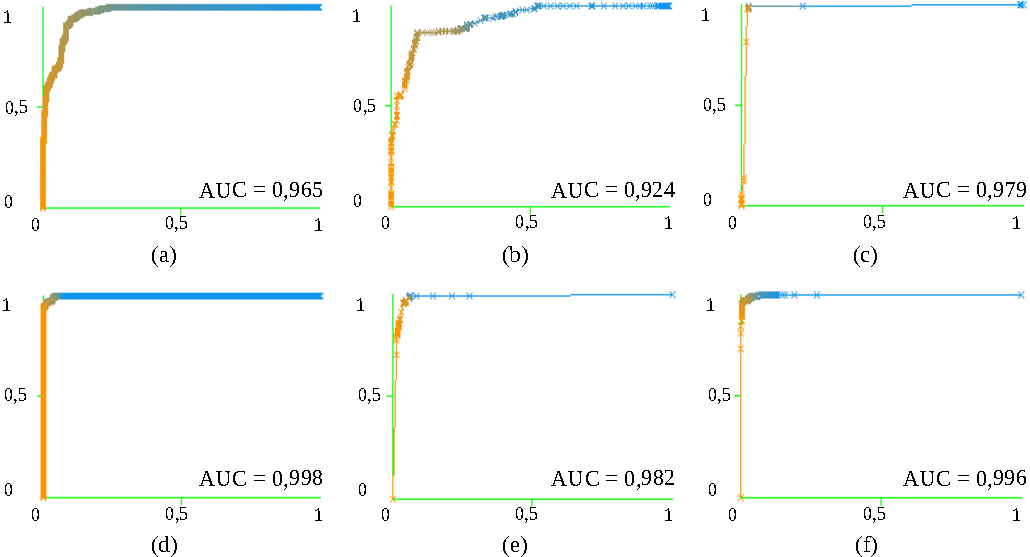
\includegraphics[scale=.85]{_fig/roc.pdf}
\caption[Curva ROC dos classificadores comparados.]{Curva ROC dos classificadores comparados.
(a)~Na\"ive-Bayes.
(b)~Bayes-Net.
(c)~kNN.
(d)~MLP-LM.
(e)~DecisionTree.
(f)~RandomForest.}
\label{fig:roc}
\end{figure}	


\subsection{Impacto da primeira fase do \system} \label{sec:exp_dbcscan}

Classificar pixel a pixel a região de interesse para análise não apenas permite remover o fundo da imagem, mas também permite reduzir o tempo de execução do algoritmo de geração de superpixels e do método de agrupamento que serão utilizados na segunda fase.
Essa redução, na realidade, se dá porque o número de \textit{entradas} para esses algoritmos é reduzida.
Por exemplo, para uma imagem não processada, a quantidade de superpixels gerados é o mesmo número de superpixels que deveriam ser agrupados na segunda fase do \system.
No entanto, ao se remover o fundo, deve-se retirar do conjunto de superpixels gerados o número correspondente aos superpixels de fundo, \textit{i.e.}, a quantidade de entrada para o algoritmo de agrupamento pode ser reduzida substancialmente.
Some-se a isso o fato que os pixels removidos geram uma região escura e sem bordas, para qual a convergência do algoritmo de geração de superpixels é facilitada, \textit{i.e.}, resolvida como uma grade comum uniformemente espaçada.

Portanto, nesse segundo experimento mediu-se o impacto da remoção de pixels de fundo ao se calcular o número de regiões de interesse (superpixels) eliminadas da segunda fase de análise do \system em função da quantidade $k$ de superpixels solicitados.
Dessa forma, foi utilizada uma taxa de descarte $[0,1]$ para medir o percentual de entradas que podem ser descartadas da segunda fase do \system ao se remover o fundo da imagem original.
A Figura~\ref{fig:efic} apresenta os valores de média e desvio padrão para cinco imagens do conjunto \dataset avaliadas considerando a proporção de regiões de interesse descartadas em função da quantidade $k$ de superpixels solicitada.
Nesse sentido, quanto maior o índice de descarte, mais eficiente é a classificação em eliminar regiões candidatas.
O resultado consolidado no gráfico de barras indica que a taxa de descarte cresce linearmente com o número de superpixels, com desvios padrões que se tornam relativamente estáveis a partir de determinado ponto.
O descarte de regiões para $k = 3 \cdot 10^3$ é, na média, superior a $10\%$ e chega até $48\%$ de eficiência para quando a quantidade de superpixels solicitadas é próxima a $10 \cdot 10^3$.

Esse resultado é particularmente importante para a aplicação do \system em domínios similares, onde a qualidade da solução pode aumentar para um número maior de superpixels, cujo valor será limitado, na prática, pelos recursos computacionais disponíveis.
	
\begin{figure}[!htb]
\centering
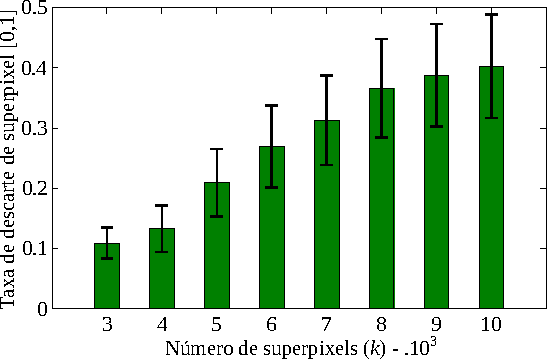
\includegraphics[scale=0.92]{_fig/efic.pdf}
\caption[Taxa de superpixels descartados pela primeira fase do \system]{Taxa de superpixels descartados pela primeira fase do \system.}
\label{fig:efic}
\end{figure}	
	
\subsection{Avaliação dos parâmetros da segunda fase do \system} \label{sec:exp_dbcscan_2}

\begin{figure}[!b]
\centering
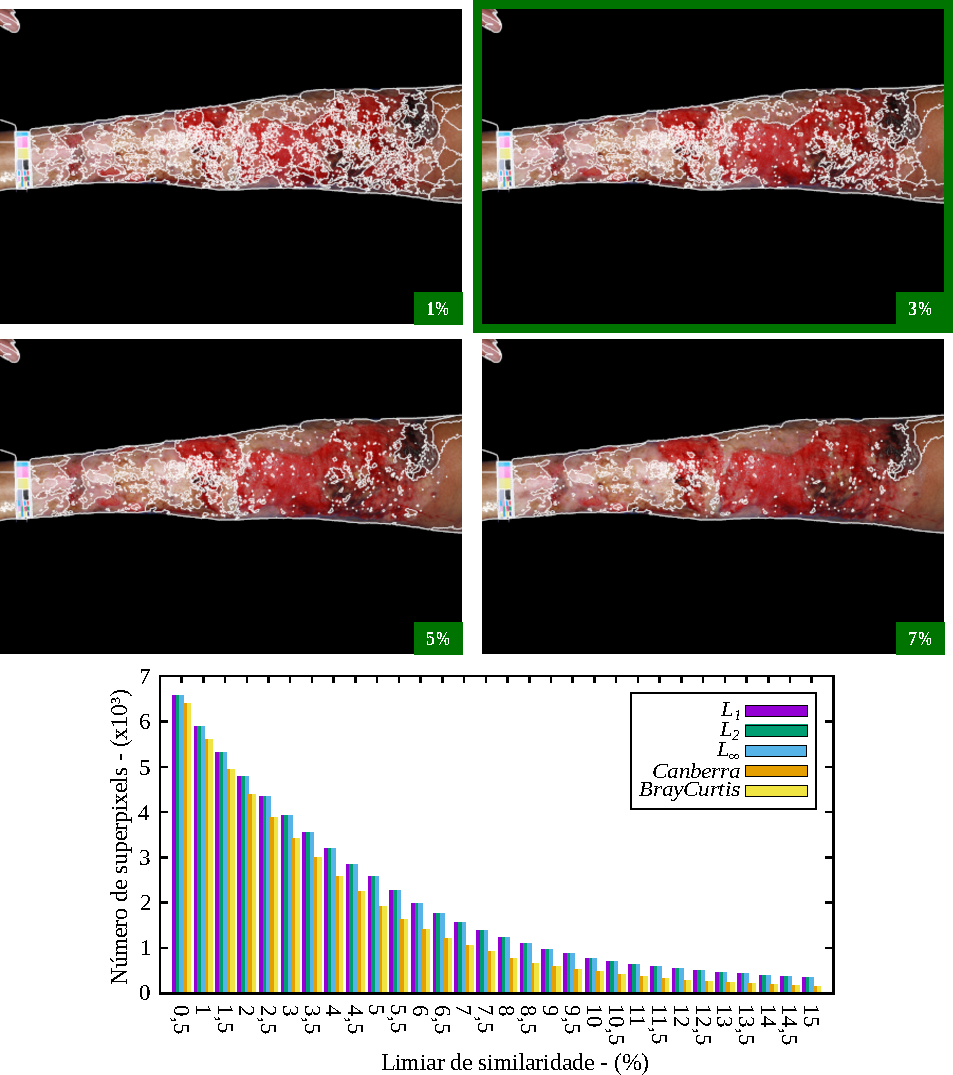
\includegraphics[scale=.93]{_fig/res1.pdf}
\caption[Primeiro exemplo de ajuste automático do \system com o uso de gráficos de barras e critério Scree-Plot.]{Primeiro exemplo de ajuste automático do \system com o uso de gráficos de barras, múltiplas funções de distância e critério Scree-Plot.}
\label{fig:expto_dbscan}
\end{figure}

Para o ajuste de parâmetros da segunda fase do \system consideramos o agrupamento dos superpixels gerados pelo algoritmo SLIC cujos representação RGB não tenha sido descartada pela primeira fase da solução.
Com relação ao algoritmo de agrupamento foi usada uma implementação do DBSCAN e os testes foram realizados sobre cinco imagens com fundo automaticamente removido pelo classificador.
Como entrada do algoritmo de agrupamento fica a imagem dividida em superpixels, cuja representação é colocada no espaço LAB que é o mais adequado para a aplicação de funções de distância, de acordo com a literatura.
Dois parâmetros do DBSCAN foram avaliados, a saber a distância máxima de similaridade $\xi$ e a função de distância.

\begin{figure}[!b]
\centering
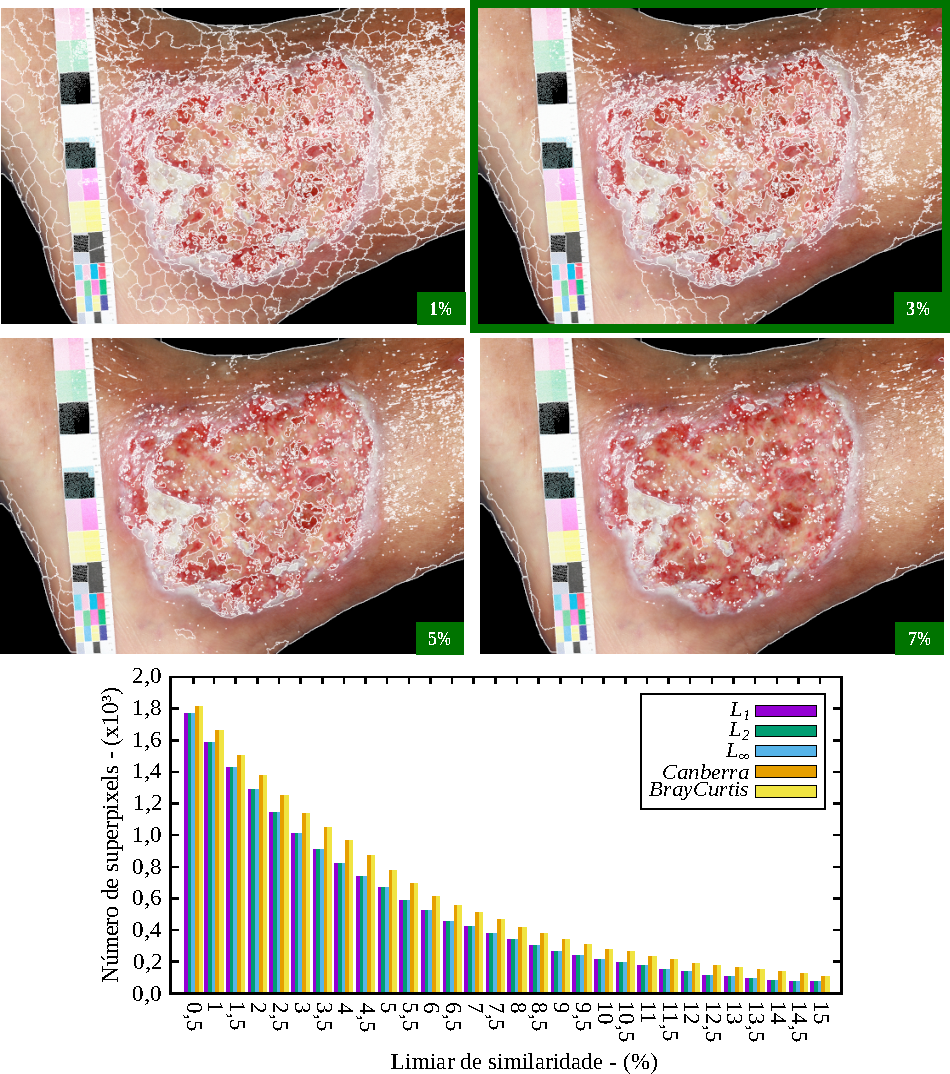
\includegraphics[scale=.93]{_fig/res2.pdf}
\caption[Segundo exemplo de ajuste automático do \system com o uso de gráficos de barras e critério Scree-Plot.]{Segundo exemplo de ajuste automático do \system com o uso de gráficos de barras, múltiplas funções de distância e critério Scree-Plot.}
\label{fig:expto_dbscan2}
\end{figure}

Em particular, foram avaliadas cinco funções de distância, sendo três da família de Minkowiski, $L_1$, $L_2$, $L_\infty$), e duas variações; Canberra e BrayCurtis. 
O intervalo de similaridade $\xi$ foi experimentado como uma variação percentual com relação ao valor de similaridade normalizada de referência do espaço LAB empregue para calcular a distância de superpixels que é de três unidades.
Assim, definiu-se $30$ intervalos para $\xi$ variando de $ 0,5\%$ até $15\%$ da distância máxima de referência, com passos percentuais de $0,5\%$, \textit{i.e.}, $\xi \in \{0,5\%, 1\%, 1,5\% \ldots, 15\% \}$.

As Figuras~\ref{fig:expto_dbscan} e ~\ref{fig:expto_dbscan2} mostram dois exemplos de segmentação geradas pelo DBSCAN e as configurações avaliadas para duas das cinco imagens testadas.
Além de resultados específicos, as figuras mostram o comportamento das funções de distância na forma de um gráfico de barras.
Esses gráficos ilustram a quantidade de grupos obtidos após a segmentação pelo DBSCAN em função do intervalo de similaridade, onde os números máximos e mínimos de grupos são completamente dependentes de cada figura.
Pelos resultados dos gráficos pode-se observar que as funções de distância Canberra e BrayCurtis foram as que apresentaram a variação mais ampla, obtendo ora a maior ora a menor quantidade de grupos, a depender da entrada.
Por outro lado, a função $L_1$ exibiu um comportamento \textit{estável}, no sentido de estar sempre entre as três funções que geram a menor quantidade de grupos por intervalo para todas as imagens avaliadas.
De fato, embora as funções da família Minkowiski tenham apresentado resultados próximos entre si, na média, a função $L_1$ foi a que gerou o menor número de grupos, na comparação com as funções $L_2$ e $L_\infty$ para as imagens analisadas.
Com base nessas observações, definiu-se a função $\delta = L_1$ como o parâmetro mais adequado para medir a similaridade entre superpixels da segunda fase da solução \system.

Outro comportamento peculiar observado pelos gráficos de barras nas Figuras~\ref{fig:expto_dbscan} e~\ref{fig:expto_dbscan2} é que o número de grupos gerados se assemelha a um decaimento exponencial em função do intervalo de similaridade, cuja inclinação se nivela em direção ao ``cotovelo'' da curva.
Esse comportamento também é observado em diversas outros problemas que requerem a definição de um número fixo de parâmetros~\cite{Jolliffe2011,Semaan2012}, como o critério de \textit{Scree-Plot} usado para a escolha da quantidade de dimensões relevantes a serem tomadas de um conjunto de dados após a transformação multidimensional de Análise de Componentes Principais.
Nesse sentido, adotou-se o critério do Scree-Plot para a escolha do parâmetro de limite de similaridade do DBSCAN a ser usado pela implementação do \system.
A premissa da escolha desse ponto de corte é que o ``cotovelo'' da curva de decaimento exponencial indica onde o gráfico de barras começa a ser suavizado.
Assim, o ponto é determinado pela primeira das duas barras consecutivas cuja razão de diferença não exceda um limite fixo $\Delta$, de acordo com a expressão na Equação~\ref{eq:limBarra}.

\begin{equation}\label{eq:limBarra}
    \Delta \leq \frac{ \text{barra}_i - \text{barra}_{i+1}}{\text{barra}_i}, i \in [0,5\%, 15\%).
\end{equation}

Foram realizados experimentos sobre o valor de $\Delta$ variando a razão de $5\%$ até $20\%$ em passos de $1\%$ e o ponto de corte mais frequente observado com relação às imagens avaliadas foi o limite de similaridade $\xi = 3\%$.
As Figuras~\ref{fig:expto_dbscan} e~\ref{fig:expto_dbscan2} mostram dois exemplos de como a variação do intervalo de similaridade impacta na qualidade da segmentação gerada pelo algoritmo de agrupamento.
Para pequenos valores de similaridade, a maior parte dos superpixels é mantida e o resultado final é de muitas regiões de interesse, o que dificulta a análise pelo especialista ou inviabiliza o cálculo da área por região lesionada (que são muitas).
Para valores muito altos de similaridades, todos os superpixels são unidos em regiões únicas, o que impede a separação de tecidos lesionados ou de cicatrização em grupos bem definidos.

Os resultados nas Figuras~\ref{fig:expto_dbscan} e~\ref{fig:expto_dbscan2} destacam as segmentações obtidas pelo DBSCAN com as configurações $\delta = L_1$ e $\xi = 3\%$ com bordas verdes, cujas regiões de interesse segmentadas apresentam uma troca entre a quantidade de grupos e a boa separação entre os tecidos.
Essa qualidade de visualização se apresentou em todas as imagens testadas com a configuração, indicando que o uso do critério Scree-Plot é adequado como compromisso entre baixo número de grupos e \textit{clusters} formados com tecidos diferentes.
Portanto, para o último experimento, será usado o método \system com sua configuração mais adequada, de acordo com todos os experimentos realizados.
A saber:

\begin{itemize}
    \item \underline{Número de superpixels $k$}, como uma razão do perímetro da área original e a taxa de $550$,
    \item \underline{Classificador $\phi$}, como uma rede neural MLP de apenas três camadas totalmente conectadas, função de ativação logística na camada intermediária e algoritmo de treinamento de Levenberg-Marquardt,
    \item \underline{Função de distância $\delta$}, como a função de distância $L_1$ e, finalmente,
    \item \underline{\textit{Threshold} de similaridade $\xi$}, como $3\%$ do valor máximo de distância em LAB.
\end{itemize}


\subsection{\system \textit{vs.} Segmentação manual -- Quantificação de áreas de interesse} \label{sec:exp_vs_especialista}


Para o último experimento foram separadas quatro imagens do conjunto de dados \dataset não testadas e/ou avaliadas anteriormente e foi solicitado a um especialista que segmentasse manualmente a lesão entre fundo, pele saudável, borda da pele e tecido lesionado por meio da ferramenta ImageJ\footnote{\url{imagej.nih.gov/ij/}}.
As Figuras~\ref{fig:quantification}(a--b) mostram uma das imagens selecionadas e a segmentação realizada manualmente pelo especialista, enquanto as Figuras~\ref{fig:quantification}(c--d) mostram as saídas geradas pela primeira e segunda fase da solução \system, respectivamente.

\begin{figure}[!t]
\centering
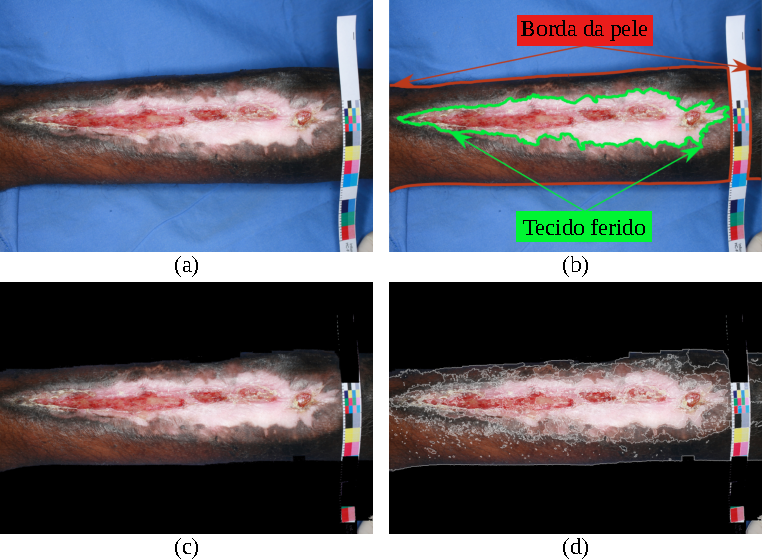
\includegraphics[scale=.9]{_fig/quantification.pdf}
\caption[Segmentação \system \textit{vs.} segmentação manual]{
Segmentação \system \textit{vs.} segmentação manual.
(a)~Exemplo de imagem do \dataset.
(b)~Segmentação manual do especialista.
(c)~Resultado da primeira fase do \system.
(d)~Resultado da segmentação do \system.}
\label{fig:quantification}
\end{figure}

Para medir a qualidade da segmentação alcançado pelo \system quando comparada com a segmentação manual fornecida pelo especialista, a mascára de saída do \system foi justaposta a imagem obtida do especialista.
Nesse sentido, a segmentação foi considerada ``correta'' quando todos os pixels de um superpixel se encaixam na mesma região segmentada pelo especialista.
A segmentação foi considerada ``parcialmente correta'' quando uma porção dos pixels do superpixel está em uma área segmentada pelo especialista e outra porção em outra área.
Nesses casos, o superpixel foi considerado do mesmo grupo da região que apresentou o casamento do maior número de pixels entre o superpixel a imagem segmentada pelo especialista.

A taxa de Erro Absoluto Médio (MAE), revisada na Seção~\ref{sec:background} e na Equação~\ref{eq:mad} pode ser facilmente ajustada para calcular a taxa de segmentação para as regiões ``corretas'' e ``parcialmente corretas''.
Nesse sentido, considera-se cada uma das regiões segmentadas pelo especialista como uma classe e os superpixels são classificados como a mesma classe do maior número de pixels casados na imagem segmentada pelo especialista.
Portanto, a taxa MAE pixel a pixel de uma imagem é a soma das menores quantidades de pixels que foram casadas em duas ou mais regiões da imagem segmentada.
De acordo com essa medida, os pixels das quatro imagens foram comparadas entre as duas segmentações com uma taxa MAE de apenas $0,05$ e variância de $0,01$, o que representa uma taxa de separação de tecidos muito próxima a gerada manualmente.

\subsection{Conclusões Parciais}

Essa seção apresentou resultados experimentais sobre a proposta \system com relação a dois cenários distintos: 
\textit{(i)}~determinar a melhor configuração de parâmetros para a solução e 
\textit{(ii)}~comparar a estratégia segmentação por divisão e conquista com a segmentação manual do especialista.
Para a avaliação foi usado o conjunto de dados \dataset com uma série extensiva de avaliações sobre diversos métodos de classificação, que culminaram por indicar o classificador MLP com três camadas e o algoritmo de aprendizado de Levenberg-Marquardt como a primeira do método \system.
Na sequência, foram avaliadas cinco funções de distância e $30$ intervalos de similaridade como parâmetros candidatos ao algoritmo de agrupamento DBSCAN.
O critério de Scree-Plot indicou o limite de similaridade de $3\%$ e a função de distância $L_1$ como os parâmetros mais adequados.
Por último, mas não menos importante, a solução \system com os parâmetros ajustados foi capaz de alcançar uma segmentação próxima a gerada manualmente por um especialista, com uma taxa de Erro Absoluto Médio de $0,05$ e variância de $0,01$.
\newpage
\thispagestyle{plain} % empty
\mbox{}


